\chapter{Example graph}
\label{sec:example-graph}

\autoref{fig:example-graph-without-refreshes} shows a snapshot of an example graph.

\autoref{fig:example-graph-with-refreshes} shows an example graph with refresh operations. Deletions of a single element (node or edge) are denoted with a red cross 
\includegraphics[scale=0.14]{patterns/delete-single}, while recursive deletions are denoted with a purple cross 
\includegraphics[scale=0.14]{patterns/delete-recursively}.

\begin{figure}[ht]
    \centering
    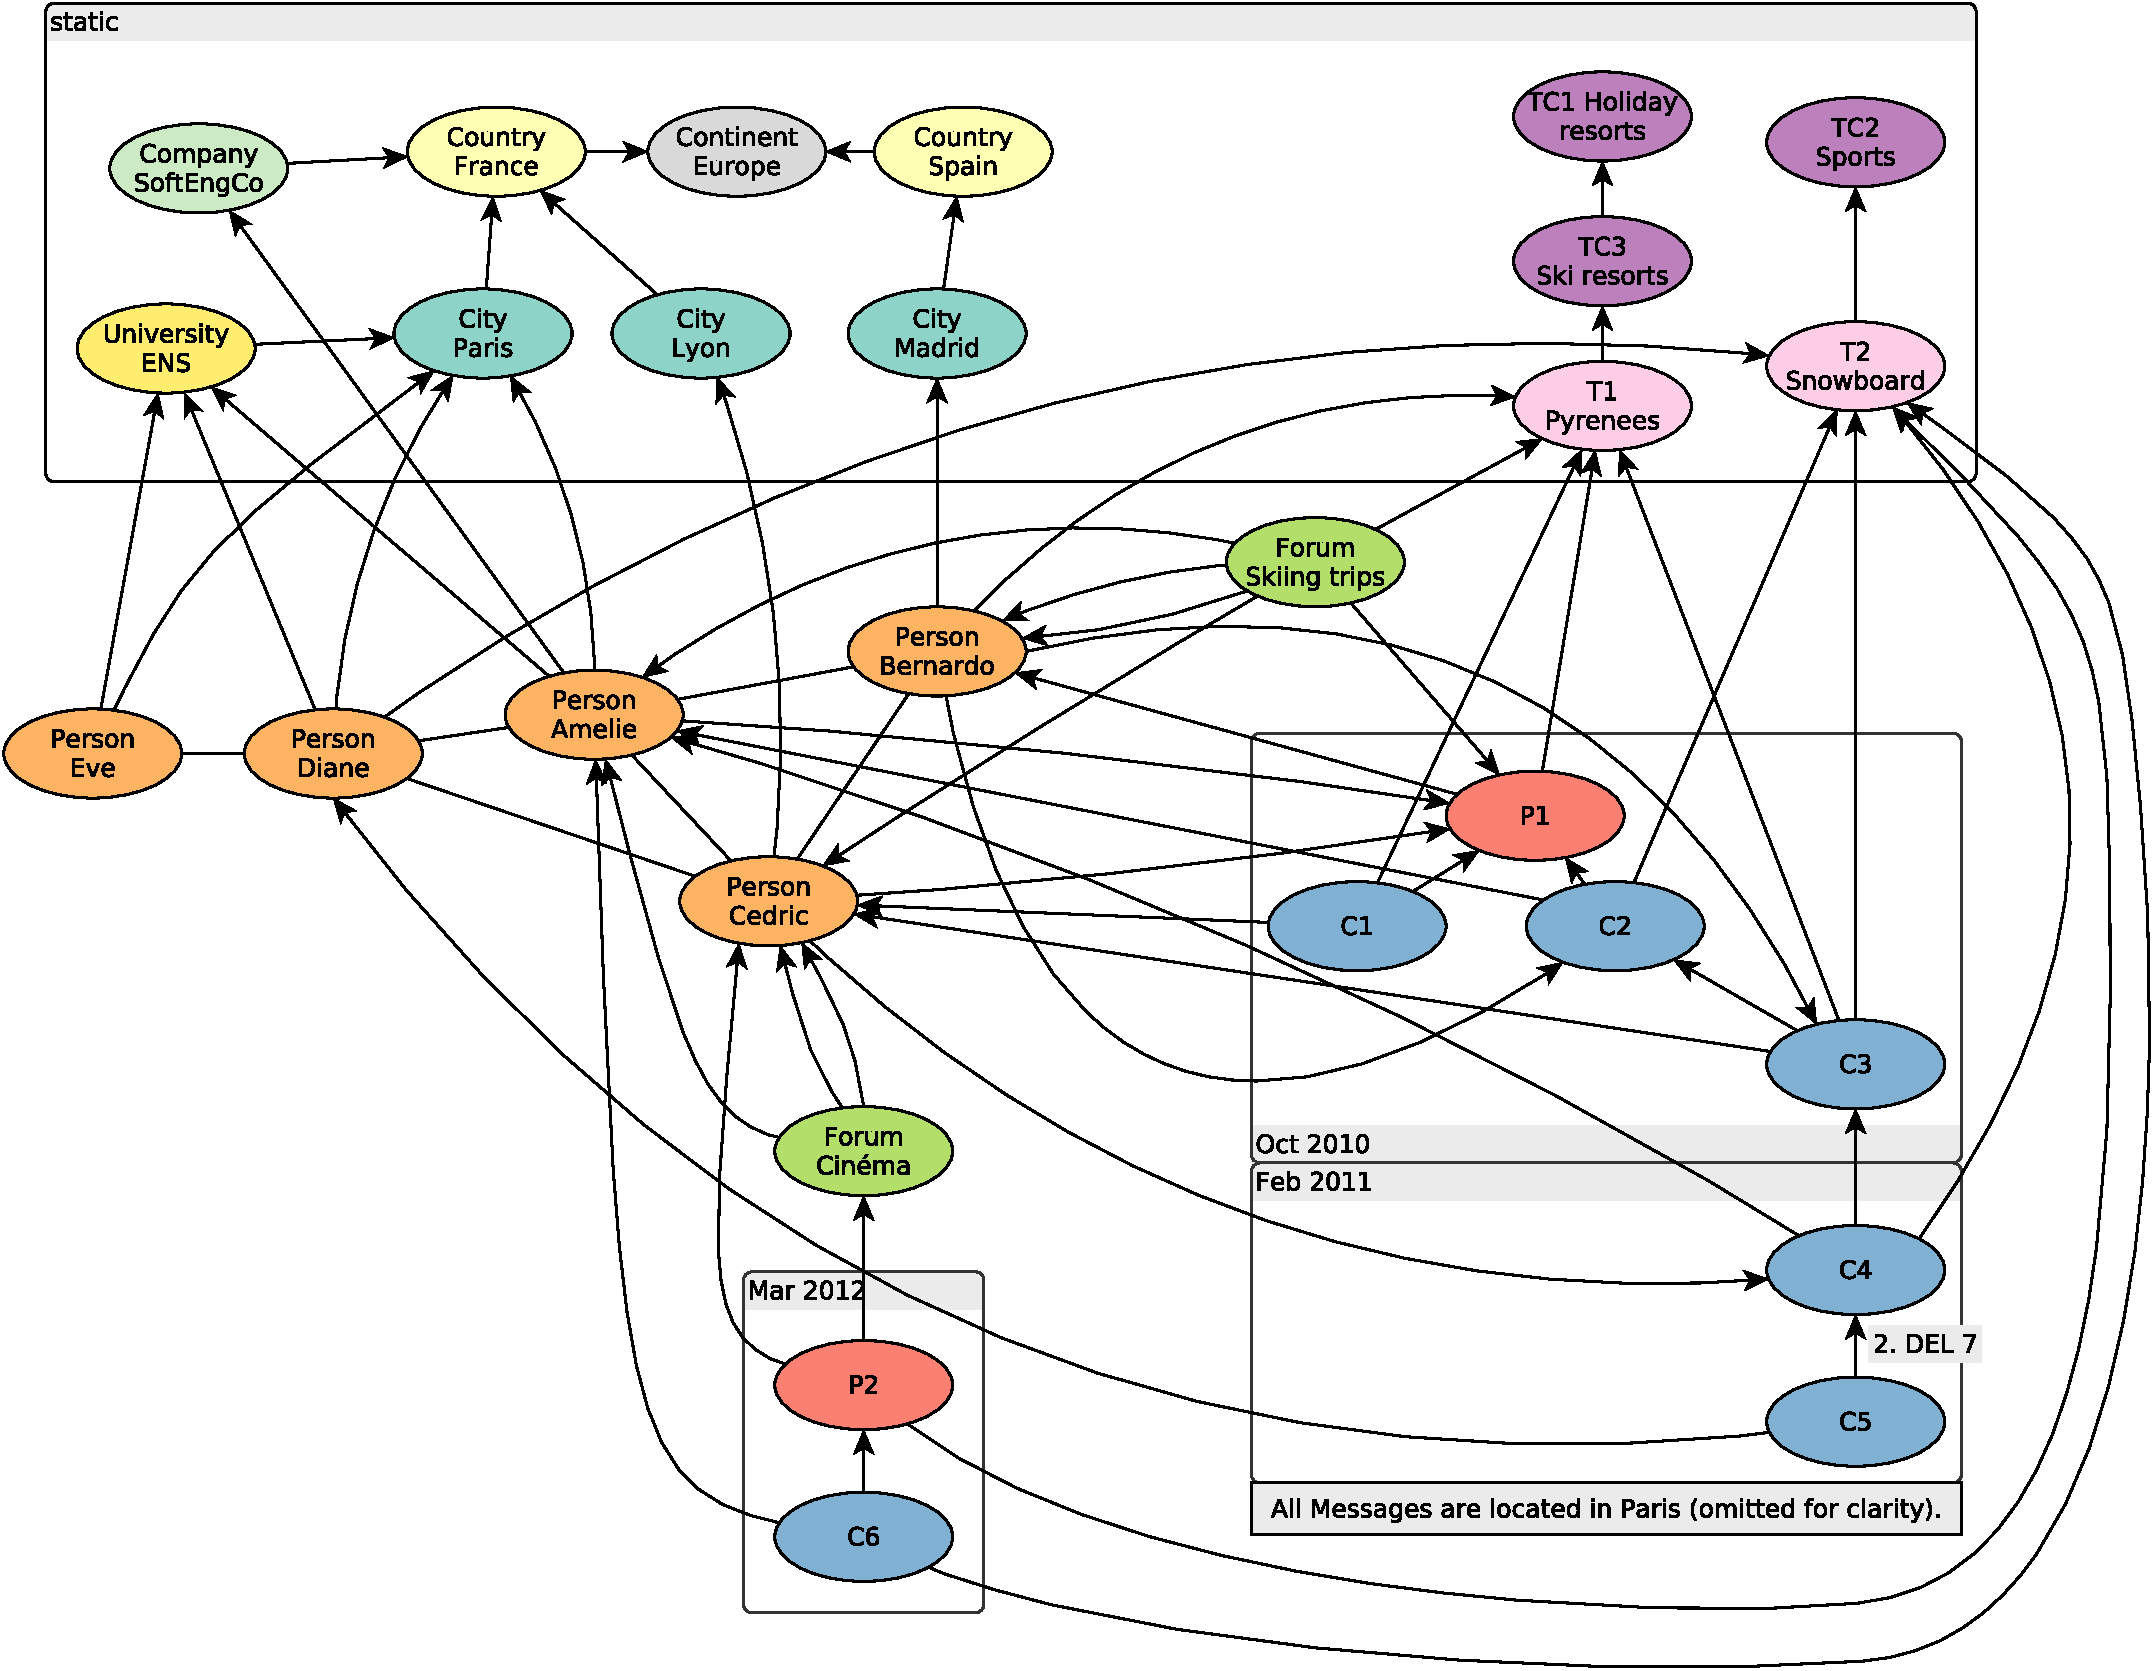
\includegraphics[scale=\yedscale]{figures/example-graph-without-refreshes}
    \caption{Example graph snapshot (without refresh operations).}
    \label{fig:example-graph-without-refreshes}
\end{figure}

\begin{figure}[ht]
    \centering
    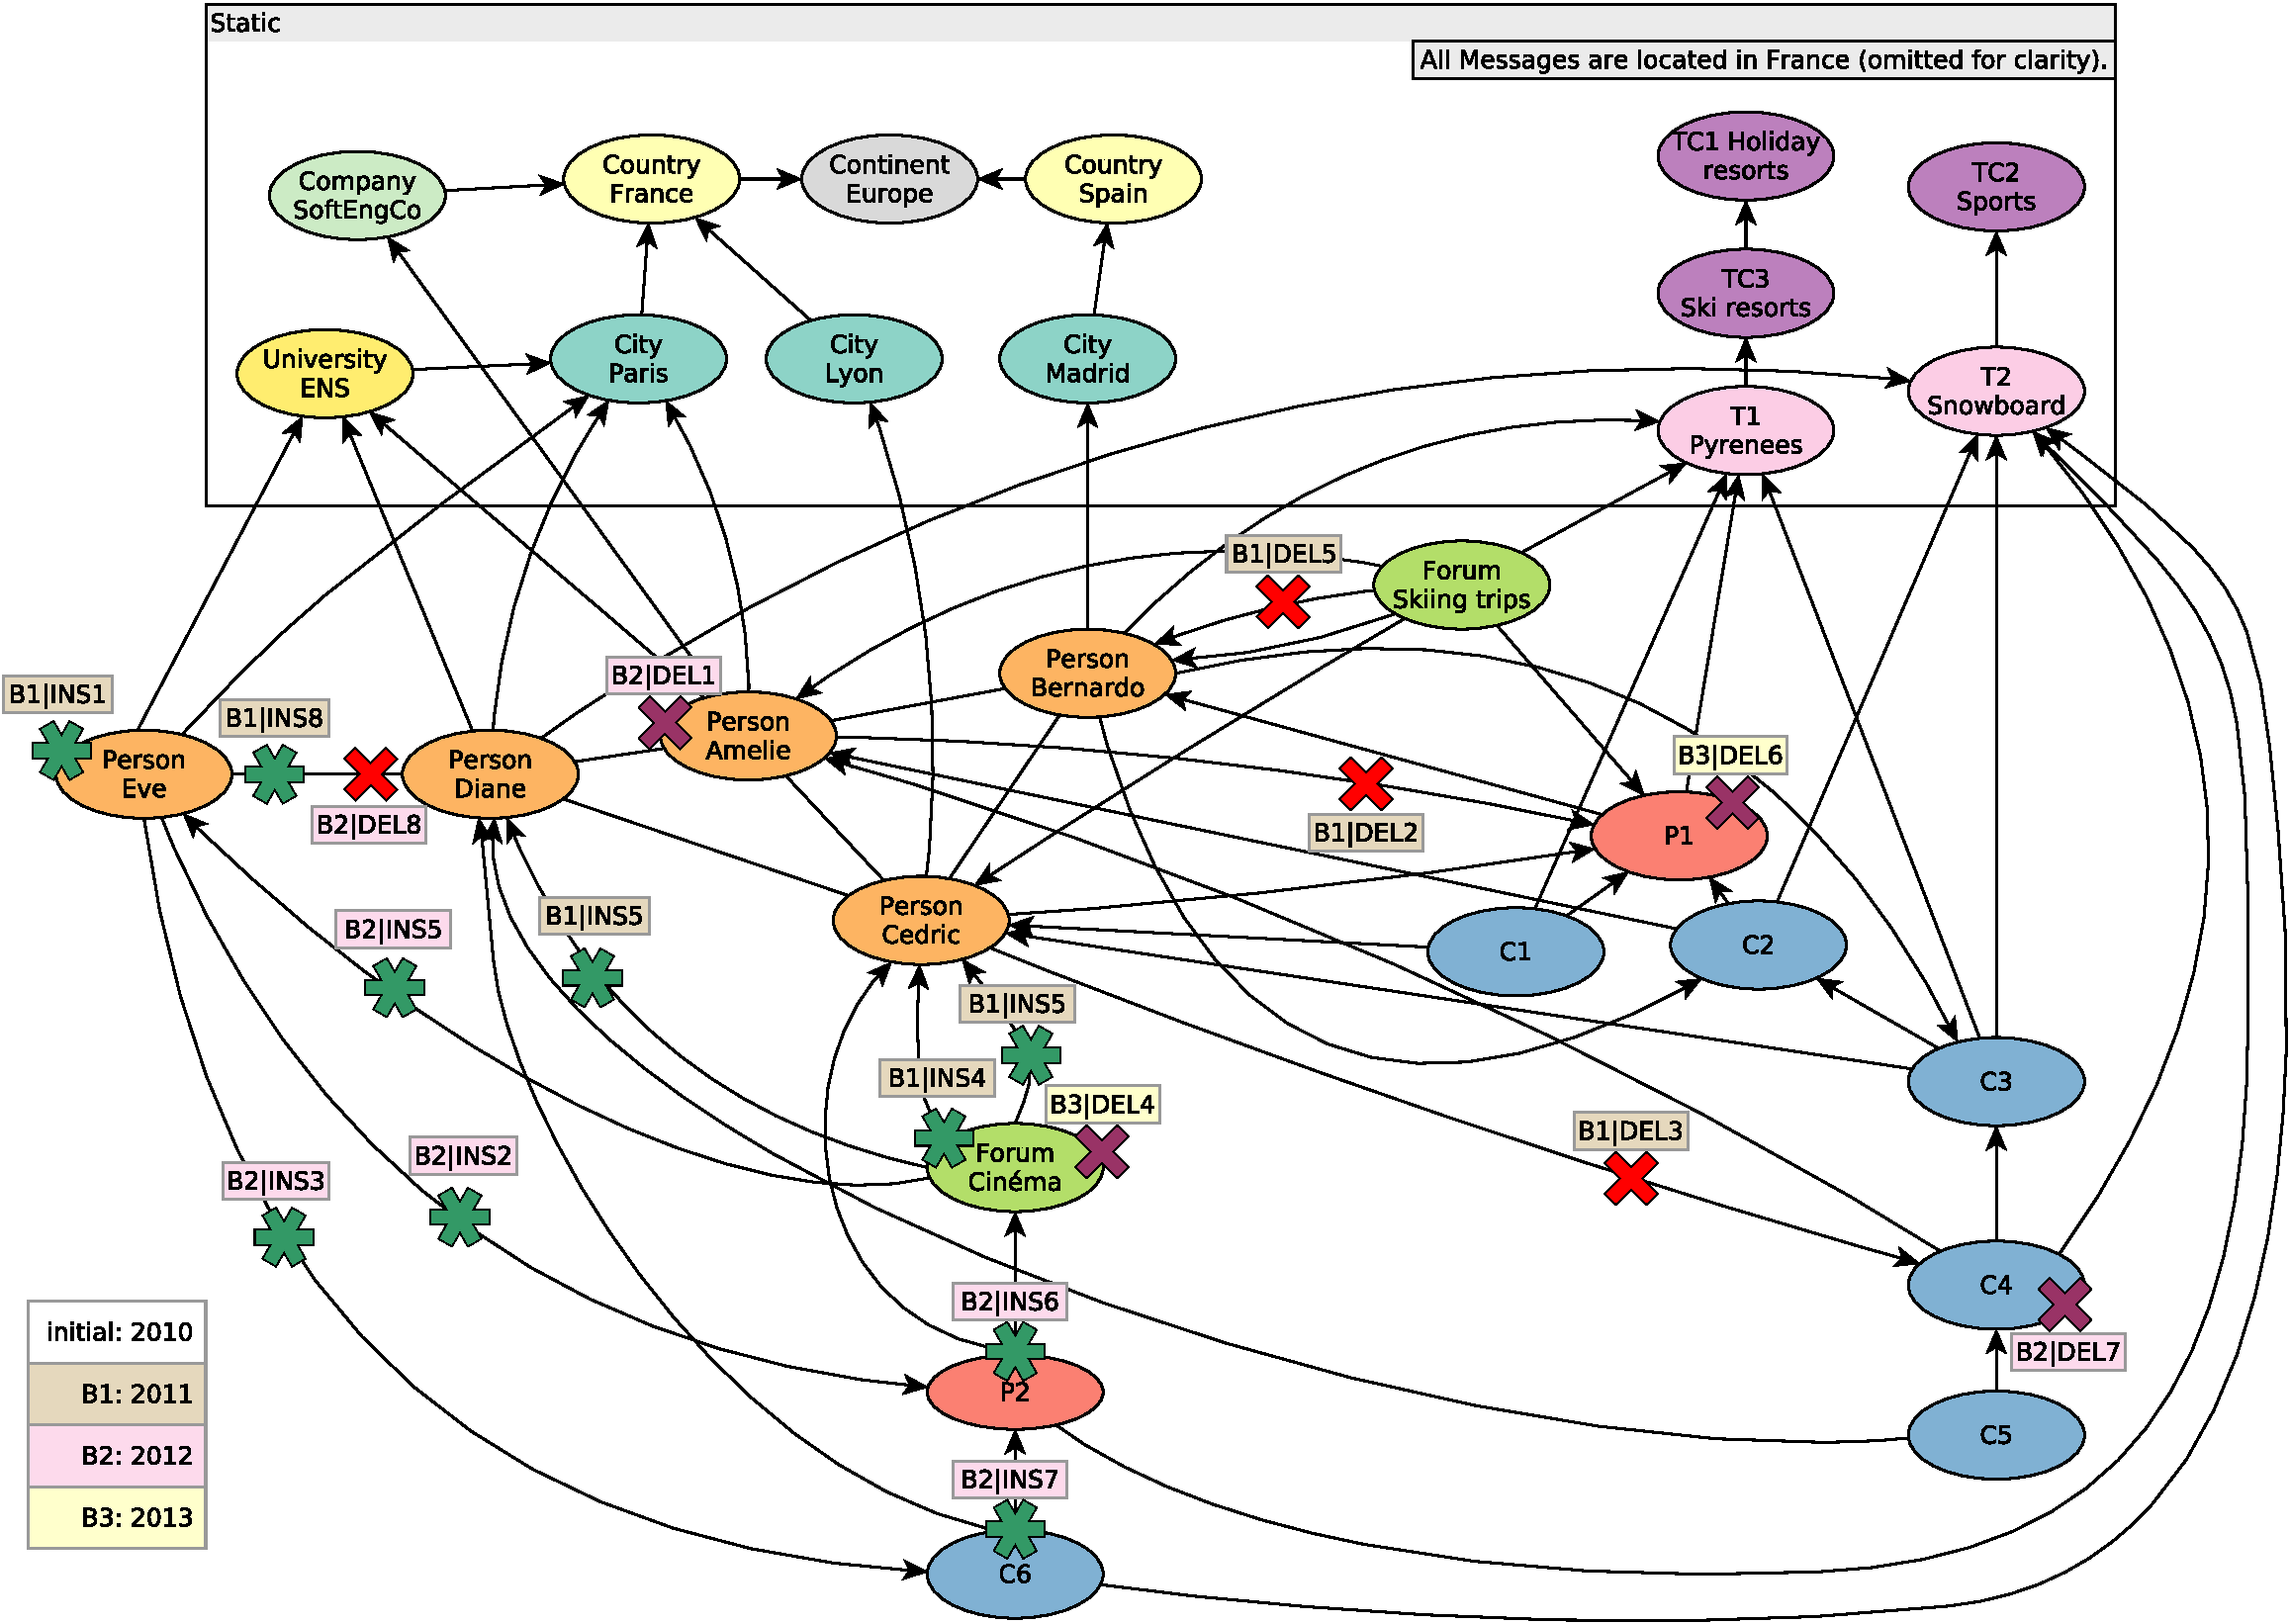
\includegraphics[scale=\yedscale]{figures/example-graph-with-refreshes}
    \caption{Example graph with refresh operations (currently deletions, inserts to be added).}
    \label{fig:example-graph-with-refreshes}
\end{figure}
